\documentclass[12pt,letterpaper]{article}
\usepackage[utf8]{inputenc}
\usepackage[english]{babel}
\usepackage{amsmath}
\usepackage{amsfonts}
\usepackage{amssymb}
\usepackage{graphicx}
\usepackage{geometry}
\usepackage{parskip}
\usepackage{mathtools} \mathtoolsset{showonlyrefs} %show only referenced equations
\usepackage{psfrag}
\usepackage[spanish,textwidth=2cm]{todonotes} %todonotes va despues de xcolor

\newcommand{\EE}{\operatorname{E}}
\newcommand{\VV}{\operatorname{Var}}

\begin{document}
\section*{Example 2.5}
A \textsl{binary noise} $X(t)$, $t \in T$, is one that takes either the value $+1$ or $-1$ throughout successive time intervals of a fixed length $\Delta$. The value it takes in one interval is independent of the value taken in any other interval; also sample functions may differ by a shift along the $t$-axis that is equally likely. The binary noise is an example of two-valued processes. A possible representation of $X(t)$ is 
\begin{equation}
X(t) = Y(t-A) \label{eq:2.57}
\end{equation}
with 
\begin{equation}
Y(t) = Y_{n},  \ \ (n-1) \Delta < t \leq n \Delta \label{eq:2.58}
\end{equation}
where the random variables $Y_n$, $n = \ldots, -2, -1, 0, 1, 2, \ldots$ are independent and identically distributed with the probability mass function 
\begin{equation}
p_{Y_n}(k) = 0.5, \ \ k = -1, 1
\end{equation}
for all $n$. The random variable $A$ in equation \eqref{eq:2.57} follows a uniform distribution in the interval $(0,\Delta)$ and is independent of $Y_n$.

A typical sample function of a binary noise is shown in Figure \ref{fig:sample_binary_noise}, where the shift $a$ is a sample value of random variable $A$.
\begin{figure}[!hb]
\centering
\psfrag{D}{$\Delta$}
\psfrag{a}{$a$}
\psfrag{X(t)}{$X(t)$}
\psfrag{t}{$t$}
\psfrag{+1}{\!$+1$}
\psfrag{-1}{\!\!\!$-1$}
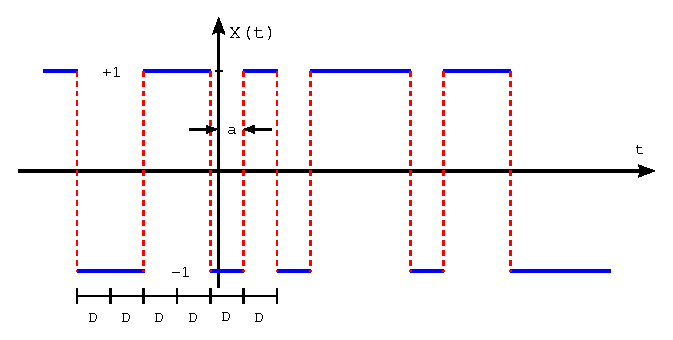
\includegraphics[width=0.8\textwidth]{sample_binary_noise.eps}
\caption{A Typical Sample Function of a Binary Noise}
\label{fig:sample_binary_noise}
\end{figure}

The mean of $X(t)$ is zero, since
\begin{equation}
\EE [X(t)] = (-1)p_{Y_n}(-1) + (+1)p_{Y_n}(1) = (-1)(0.5) + (+1)(0.5) = 0;
\end{equation}
its mean squared is
\begin{equation}
\EE[X(t)^2] = (-1)^2 p_{Y_n}(-1) + (1)^2 p_{Y_n}(1) = (-1)^2 (0.5) + (+1)^2(0.5) = 1,
\end{equation}
and its variance is
\begin{equation}
\VV[X(t)] = \EE[X(t)^2] - \EE[X(t)]^2 = 1 - 0 = 1.
\end{equation}

Consider now the correlation function $R(t_1, t_2)$. It is also clear that: 
\begin{equation}
R(t_1, t_2) = \EE\left[X(t_1) X(t_2)\right] =0, \ \ \left|t_2 - t_1 \right| > \Delta \label{eq:2.60}
\end{equation} 
due to independence of $X(t_1)$ and $X(t_2)$ when $t_1$ and $t_2$ are in different intervals. For $\left|t_2 - t_1 \right| \leq \Delta$, whether or not $X(t_1)$ and $X(t_2)$ are situated in the same interval depends upon the value $A$ takes. Then, either (see Figure~\ref{fig:cases_binary_noise}),
\begin{figure}[!hb]
\centering
\psfrag{Yn}{$Y_n$}
\psfrag{Yn1}{$Y_{n+1}$}
\psfrag{D}{$\Delta$}
\psfrag{T}{$\tau$}
\psfrag{t1}{$t_1$}
\psfrag{t2}{$t_2$}
\psfrag{(n-1)D}{$(n-1)\Delta$}
\psfrag{nD}{$n\Delta$}
\psfrag{(n+1)D}{$(n+1)\Delta$}
\psfrag{case 1}{case 1}
\psfrag{case 2}{case 2}
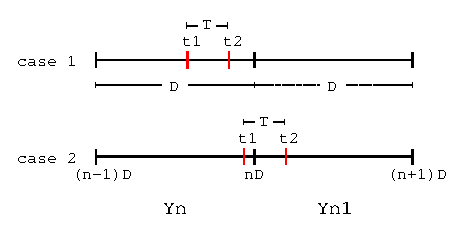
\includegraphics[width=0.8\textwidth]{cases_binary_noise.eps}
\caption{$t_1$ and $t_2$ in the same or in different time intervals.}
\label{fig:cases_binary_noise}
\end{figure}
\begin{itemize}
 \item Case 1 - $X(t_1)$ and $X(t_2)$ are in the same interval: in this case, $X(t_1) = X(t_2) = Y_n$ happens with probability $P\left\{ A \leq \Delta - \left| t_2-t_1 \right| \right\} = \frac{\Delta - \left| t_2-t_1 \right|}{\Delta} = 1 - \frac{\left| t_2-t_1 \right|}{\Delta}$ or,
 \item Case 2 - $X(t_1)$ and $X(t_2)$ are different intervals: in this case, $X(t_1) = Y_n$ and $X(t_2) = Y_{n+1}$  happens with probability $P\left\{ A > \Delta - \left| t_2-t_1 \right| \right\} = \frac{\left| t_2-t_1 \right|}{\Delta}$.
\end{itemize}

Hence, if $\left|t_2 - t_1\right| \leq \Delta$ then
\begin{align}
R(t_1,t_2) &= \EE\left[X(t_1) X(t_2)\right] \\
&= \EE\left[Y(t_1 - A) Y(t_2-A)\right] \\
&= \EE\left\{Y_n^2  \right\} P\left\{ A \leq \Delta - \left| t_2-t_1 \right| \right\} + \EE\left\{Y_n Y_{n+1}  \right\} P\left\{ A > \Delta - \left| t_2-t_1 \right| \right\}\\
&= (1)\left(1-\frac{\left|t_2-t_1\right|}{\Delta}\right) + (0)\left(\frac{\left|t_2-t_1 \right|}{\Delta}\right) \\
&= 1 - \frac{\left| t_2-t_1 \right|}{\Delta} \label{eq:2.61}
\end{align}

Combining equations \eqref{eq:2.60} and \eqref{eq:2.61} and setting $t_2 - t_1 = \tau$, we have
\begin{equation}
R(t_1, t_2) \equiv R(t_2 - t_1) = R(\tau) =
\begin{cases}
1- \frac{|\tau|}{\Delta} & \text{if } |\tau| \leq \Delta \\ 
0                        & \text{if } |\tau| > \Delta;
\end{cases}
\end{equation}
this autocorrelation function has a triangular shape, as shown in Figure \ref{fig:correlation_binary_noise}. It also follows that a binary noise is a weakly stationary stochastic process. 
\begin{figure}
\centering
\psfrag{+D}{$+\Delta$}
\psfrag{-D}{$-\Delta$}
\psfrag{T}{$\tau$}
\psfrag{1}{1}
\psfrag{R(T)}{$R(\tau)$}
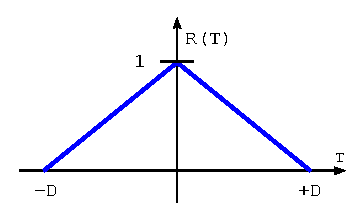
\includegraphics[width=0.5\textwidth]{correlation_binary_noise.eps}
\caption{Correlation function of a binary noise}
\label{fig:correlation_binary_noise}
\end{figure}

As a more general case, if random variables $Y_n$ in equation~\eqref{eq:2.58} are independent random variables with mean zero and variances $\sigma^2$, the correlation function has the form 
\begin{equation}
R(\tau) =
\begin{cases}
\sigma^2\left(1- \frac{|\tau|}{\Delta}\right) & \text{if } |\tau| \leq \Delta \\ 
0                                             & \text{if } |\tau| > \Delta.
\end{cases}
\end{equation}


\section*{Example 2.6}
Another important two-valued stochastic procccess is the \emph{random telegraph signal.} It has the properties that its values are +1 or -1 at successive intervals, and the time instants at which the values change obey a Poisson distribution. In mathematical terms, the random telegraph signal can be represented by 
\begin{equation}
X(t)=A(-1)^{Y(t)} 
\end{equation}
where $Y(t)$ is a \emph{Poisson counting process} to be discussed in more detail in Example 2.18, which has the properties that, for $t_1 < t_2 < t_3 < t_4$, the random variables $Y(t_2)-Y(t_1)$ and $Y(t_4)-Y(t_3)$ are independent and 
\begin{equation}
P\left[Y(t+\tau) - Y(t) = k \right] = \frac{(\lambda\tau)^k\exp(-\lambda\tau)}{k!} \ \ \text{for } k=0, 1, 2, \ldots \label{eq:PDFY2Y1}
\end{equation}
The random variable $A$ is independent of $Y(t)$, and it is distributed according to
\begin{equation}
p_A(k) = 0.5 \ \ \text{for } k = -1, 1;
\end{equation}
it is easy to deduce that $\EE_A[a] = 0$ and $\VV_A[a] = 1$.

A typical sample function of the random telegraph signal is shown in Figure~\ref{fig:sample_random_telegraph_signal}.
\begin{figure}[hb]
\centering
\psfrag{X(t)}{$X(t)$}
\psfrag{t}{$t$}
\psfrag{+1}{\!\!\!$+1$}
\psfrag{-1}{\!$-1$}
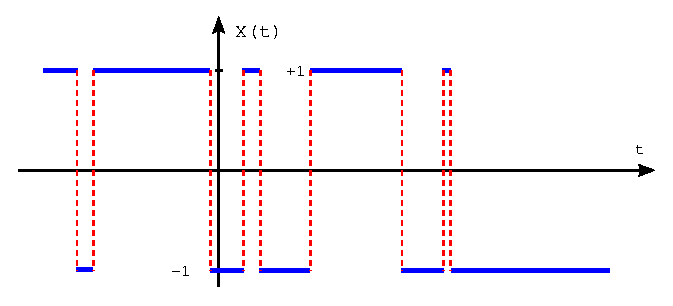
\includegraphics[width = 0.8 \textwidth]{sample_random_telegraph.eps}\\
\caption{A typical sample function of the random telegraph signal.}
\todo[inline]{Falta simular adecuadamente esta realizaci\'on utilizando procesos de Poisson.}
\label{fig:sample_random_telegraph_signal}
\end{figure}

This stochastic process has a zero mean, since
\begin{align}
\EE[X(t)] &= \EE_{AY}\left[A(-1)^{Y(t)}\right] \\
&= \sum_{a=\{-1,1\}}\sum_{y=0}^\infty a(-1)^y p_A(a) p_Y(y) \\
&= \underbrace{\sum_{a=\{-1,1\}} a p_A(a)}_{\EE_A[a] = 0} \underbrace{\sum_{y=0}^\infty  (-1)^y p_Y(y)}_{\EE_Y[(-1)^{y(t)}]} \\
&= 0;
\end{align}
also it has a correlation function
\begin{align}
R(t_1,t_2)
&= \EE_{AY}\left[X(t_1)X(t_2)\right] \\
&= \EE_{AY}\left[A(-1)^{Y(t_1)} A(-1)^{Y(t_2)} \right] \\
&= \EE_{AY}\left[A^2(-1)^{Y(t_1) + Y(t_2)} \right] \\
&= \underbrace{\EE_{A}\left[A^2\right]}_{= 1} \EE_{Y}\left[(-1)^{Y(t_1) + Y(t_2)} \right] \\
&= \EE_{Y}\left[(-1)^{Y(t_2) - Y(t_1) + 2Y(t_1)} \right] \\
&= \EE_{Y}\left[(-1)^{Y(t_2) - Y(t_1)} \times (-1)^{2Y(t_1)} \right]
\intertext{and since $Y(t)$ is an stochastic process with independent increments,}
&= \EE_{Y}\left[(-1)^{Y(t_2) - Y(t_1)}\right] \EE\left[(-1)^{2Y(t_1)} \right]
\end{align}
because $Y(t_2) - Y(t_1)$ and $Y(t_1)$ are independent events; also, notice that $2Y(t_1)$ is an even number, therefore $\EE\left[(-1)^{2Y(t_1)}\right] = 1$, and in consequence $R(t_1,t_2) = \EE_{Y}\left[(-1)^{Y(t_2) - Y(t_1)}\right]$. Taking into account that $t_2 = t_1 + \tau$, we may write 
\begin{align}
R(t_1,t_1 + \tau) 
&= \EE_{Y}\left[(-1)^{Y(t_1 + \tau) - Y(t_1)}\right]\\
&= \sum_{k=0}^\infty (-1)^k \frac{(\lambda|\tau|)^k\exp(-\lambda|\tau|)}{k!} \ \ \text{(according to equation~\eqref{eq:PDFY2Y1})} \\
&= \underbrace{\sum_{k=0}^\infty \frac{(-\lambda|\tau|)^k}{k!}}_{\substack{\text{Taylor series expansion} \\ \text{of }\exp(-\lambda|\tau|)}} \exp(-\lambda|\tau|) \\
&= \exp(-2\lambda |\tau|);
\end{align}
that is, the autocorrelation function is 
\begin{equation}
R(\tau) = \exp(-2\lambda |\tau|)
\end{equation}
and in consequence the random telegraph signal is a weakly stationary stochastic process.
\end{document}